\documentclass[a4paper, fontsize=14pt]{article} \usepackage{course_work}
\bibliography{course_work.bib} %\usepackage{graphs/gnuplot-lua-tikz}
%\setcounter{page}{4} %в зависимости от того, какой по счёту страницей должно
%быть оглавление!
%\usepackage{pstricks}
\begin{document} \includepdf[pages=1-3]{cover.pdf} \newpage \tableofcontents
	\newpage \section*{Введение} 
	\addcontentsline{toc}{section}{Введение}
	
	
	\newpage 
	\section{Постановка задачи} 
	\begin{figure}[h]
		
		\centering
		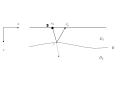
\includegraphics{migration_fig.pdf}

		\caption{Модель среды}
		\label{fig:mig}
	\end{figure}
 	Рассмотрим задачу нахождения значения скалярного волнового поля на поверхности наблюдения.
 	Допустим задана поверхность, ограничивающая некоторую область пространства $D=[0,X]\times [0,Y]\times [0,Z]$, изображённую на рисунке \ref{fig:mig}.
 	Область пространства $D$ разделена на слои $D_1$ и $D_2$, с постоянной скоростью звука $c_1$ и $c_2$ соответственно.
 	На границе находятся точечные источники колебаний $S$, которые возбуждают акустическую волну.
 	
 	Необходимо по данным характеристикам источников найти значение волнового поля на поверхности наблюдения $z=Z$.
	
	\section{Волновое уравнение}
	Конечно, решение данной задачи можно получить при помощи решения дифференциального волнового уравнения \ref{eq:wav}. 
	\begin{equation}
		\frac{\partial^2 P}{\partial x^2} + \frac{\partial^2 P}{\partial y^2} + \frac{\partial^2 P}{\partial z^2} - \frac{1}{c^2} \frac{\partial^2 P}{\partial t^2} = F(x,y,z,t)   
	\label{eq:wav}	
	\end{equation}
	Однако, для волнового уравнения с произвольной правой частью $F(x,y,z,t)$ можно записать формулу представления решения 
	в аналитическом виде.
	\begin{equation}
		P(\bar{r}',t')=\iiint\limits_{D_1} \int\limits_{-\infty}^{+\infty} F(\bar{r},t) G(\bar{r}',t'|\bar{r},t)\,dt\,dv
	\end{equation}
	%%%%%%%%%%%%%%%%%%%%%%%%%%%%%%%%%%%
	\section{Функция Грина} 

Рассмотрим мгновенный точечный источник колебаний. Тогда правая часть уравнения \ref{eq:wav} будет иметь вид $f(x,z,t) = \delta(t)\delta(x)\delta(z)$.
$$
G(r',t'|r,t)=\begin{cases}
	\frac{1}{2\pi}\cdot\frac{1}{\sqrt{(t'-t)^2-\frac{|r-r'|^2}{c^2}}},  &|r-r'|\leq c(t'-t)\\
	0, &|r-r'|>c(t'-t)
\end{cases}
$$
\textbf{TODO} написать вывод функции Грина
	
	\section{Формула Кирхгофа}
	Так как область $D$ ограничена и имеет кусочно-гладкую границу, тогда по теореме Остроградского-Гаусса можно выразить решение в виде 
	$$
	P(r',t') = \iint\limits_{S} \int\limits_{-\infty}^{+\infty} 
	[G(r',t'|r,t)\partial_n P(r,t) 
	- P(r,t)\partial_n G(r',t'|r,t)] dt\,ds
	$$
	% 
	\textbf{TODO} написать вывод интеграла кирхгофа
	
	

	

	
	
	\clearpage
	
	
	\section*{Заключение} \addcontentsline{toc}{section}{Заключение}
	
	\newpage
	
	\addcontentsline{toc}{section}{Список литературы}
	
	\printbibliography
	
	\newpage
	
	\includepdf[pages=11]{cover.pdf}
	
\end{document}

